\section{Termpot}\label{sec:termpot}

O Termpot (ver Figura \ref{fig:termpot}) é um ambiente adaptado, com base no ambiente \emph{Wavepot}.

Comandos utilizam a sintaxe da linguagem \emph{coffeescript}\cite{burnham2011coffeescript}\footnote{\url{http://coffeescript.org/}, acessado em \today.}, que possibilita otimizações diversas, entre elas, o tempo de produção do próprio código. Neste sentido, o ambiente possibilita a improvisação de códigos com a extensão média de uma linha (ver Código \ref{code:resultado1}). 

\begin{figure}[!h]
\centering
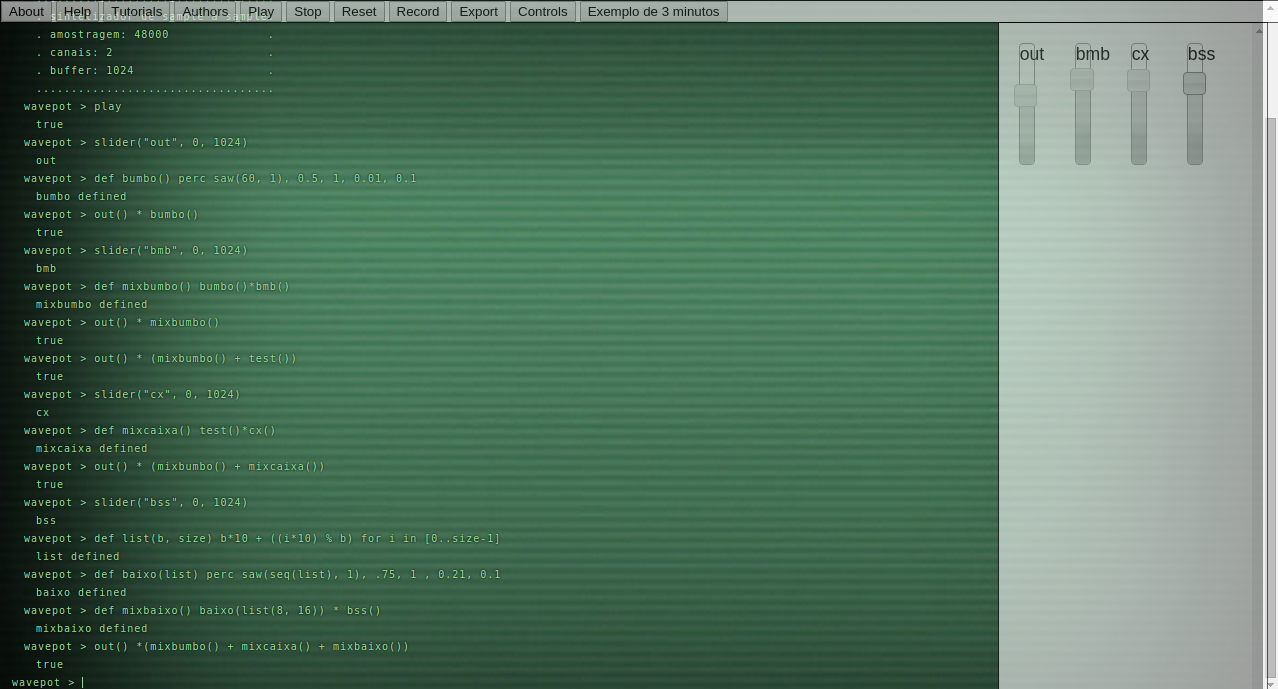
\includegraphics[scale=0.35]{termpot.png}
\caption{Aplicativo \emph{Termpot}. \textbf{Fonte}: autores.}
\label{fig:termpot}
\end{figure}

\begin{listing}
\begin{minted}[linenos,frame=lines,framesep=2mm,fontsize=\scriptsize]{javascript}
..........................................(0)
. Virtual machine started at             .
. Thu Sep 03 2015 13:32:15 GMT-0300 (BRT).
. type help for instructions             .
..........................................
$\$$ |                                    (1)
$\$$ wavepot 1024                         (2)
..................................
. sintetizador de sample a sample.        (3) 
. amostragem: 44100              .
. canais: 2                      .
. buffer: 1024                   .
..................................
wavepot > play                            (4)
wavepot > 0.71 * sin 440                  (5)
true                                      (6)
\end{minted}
\caption{Mensagem de inicialização do sistema (0). Console do \emph{Termpot} aguardando dados de entrada do improvisador (1). O improvisador inicia o ambiente \emph{wavepot} com um buffer de 1024 amostras por ciclo de DSP (2). Informações diversas do sistema de áudio inicializado (3). O improvisador inicia o processamento de áudio (4). O improvisador define o processamento de áudio (5). O sistema informa que o processamento ocorreu sem problemas (6).}
\label{code:resultado1}
\end{listing}

É interessante notar aqui um princípio de compilação \emph{Just In Time} \cite{aycock_brief_2003}. Antes que uma função de áudio específica seja executada, o sistema é executado. Ao definir uma função de saída, o sistema automaticamente a executa.

\subsection{Criação de funções em tempo de execução}

Uma das potencialidades do \emph{Termpot} é a capacidade de definir novas funções em tempo de execução. Do ponto-de-vista dos desenvolvedores, de maneira bastante rápida (não habilitamos ainda uma versão apropriada para testes com um público). 

Estas funções são escritas com o tamanho médio de uma linha, e podem ser encapsuladas em outras funções. Existem também funções de base, como \emph{noise} (Ruído branco), \emph{sin} (senóide), \emph{saw} (dente-de-serra), \emph{tri} (triangular), \emph{pulse} (pulso), \emph{env} (envelope) e \emph{seq} (sequenciamento). 

\begin{listing}
\begin{minted}[linenos,frame=lines,framesep=2mm,fontsize=\scriptsize]{javascript}
wavepot > def sin3(f, f1, f2, a) a * sin f, sin2(f1, f2)
true
wavepot > def sin2(f1, f2) sin f1, sin(f2, 0.5)
true
wavepot > inspect sin3
var tresAM;

tresAM = function(f, f1, f2, a) {
  return a * sin(f, sin2(f1, f2))
};
wavepot > inspect sin2
var doissin;

doissin = function(f1, f2) {
  return sin(f1, sin(f2, 0.5))
};
wavepot > tresAM 440, 330, 220, 0.71
true
\end{minted}
\label{code:resultado2}
\end{listing}

Além da prototipação de funções, habilitamos a criação dinâmica de GUIs de controle (\emph{sliders}, ver Código \ref{code:resultado3})

\begin{listing}
\begin{minted}[linenos,frame=lines,framesep=2mm,fontsize=\scriptsize]{javascript}
wavepot > slider "left", 0, 1024
true
wavepot > slider "right", 0, 1024
true
wavepot > stereo sin(440,0.5)*left(), sin(330, 0.5)*right()
true
\end{minted}
\caption{Exemplo de código do Wavepot}
\label{code:resultado3}
\end{listing}

Esta abordagem dos controles gráficos... TODO

%\subsection*{Metodologia de desenvolvimento}

%Para a implementação, três tarefas foram necessárias: \begin{description}
%\item[1) Customizar um emulador terminal]
%\item Utilizamos a biblioteca \emph{Ptty.js} é uma biblioteca documentada e pode ser facilmente implementada seguindo instruções de seu arquivo \emph{README}. É baseada em jQuery e permitiu uma rápida prototipação.
%\item[2) Implementar um ambiente de síntese sonora integrado ao emulador]
%\item Uma das facilidades do \emph{Ptty} é definir ambientes; elaboramos um ambiente que controla a \emph{Web Audio API} nos moldes descritos na Seção 2.
%\item[3) Comandos diversos]
%\item Ajuda, inspeção de funções, definição de novas funções, tocar, parar, pausar, gravar e download e criação de controles gráficos. Para gravação, utilizamos o \emph{recorderWorker.js}\footnote{\url{https://github.com/mattdiamond/Recorderjs/blob/master/recorderWorker.js}.} de Matt Diamond.
%\end{description}
